\section{Desenvolvimento do Algoritmo}\label{sec:figs}

O algoritmo de Dijkstra é empregado para resolver o problema.
O pseudo-código é dado a seguir:

\begin{enumerate}
    \item Inicializar todos os nós com distância infinita, exceto o nó origem $s$ que recebe 0.
    \item Marcar todos os nós como não visitados.
    \item Selecionar o nó não visitado com menor distância atual.
    \item Atualizar as distâncias dos vizinhos, se o novo caminho for mais curto.
    \item Repetir até que todos os nós tenham sido visitados ou que o destino $t$ tenha sido alcançado.
\end{enumerate}

A seguir, ilustra-se um exemplo de rede com grafo simples:

\begin{center}
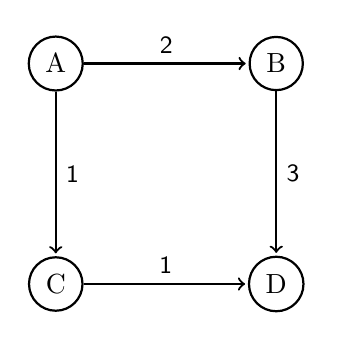
\begin{tikzpicture}[->,shorten >=1pt,auto,node distance=2.8cm,
  thick,main node/.style={circle,draw}]

  \node[main node] (A) {A};
  \node[main node] (B) [right of=A] {B};
  \node[main node] (C) [below of=A] {C};
  \node[main node] (D) [below of=B] {D};

  \path[every node/.style={font=\sffamily\small}]
    (A) edge node {2} (B)
        edge node {1} (C)
    (B) edge node {3} (D)
    (C) edge node {1} (D);
\end{tikzpicture}
\end{center}

No exemplo acima, o algoritmo de Dijkstra encontrará o caminho $A \rightarrow C \rightarrow D \rightarrow B$ ou $A \rightarrow B$ dependendo dos pesos atribuídos.
